\documentclass{nthuthesis}

\usepackage{times}
\usepackage{verbatim}
\usepackage{color}
\usepackage{url}
\usepackage{graphicx}
\usepackage{subfigure}
\usepackage{array}
\usepackage{wallpaper} 
\usepackage{cite}
\usepackage{caption}
\usepackage{float}
\usepackage{blindtext}

\usepackage{multirow}
\usepackage{makecell}
\usepackage{hhline}
\usepackage{rotating}
\usepackage{amsmath}
\usepackage{amssymb}
\usepackage{mathrsfs}

% declare the path(s) where your graphic files are
\graphicspath{{./figsrc/}}

% and their extensions so you won't have to specify these with
% every instance of \includegraphics
\DeclareGraphicsExtensions{.pdf,.jpeg,.png}

% Using the tex-text mapping for ligatures etc.
\defaultfontfeatures{Mapping=tex-text}

% Set the default fonts

% English font
% Note: please refer to 'fc-list :outline -f "%{family}\n"' for choosing a valid font name
\setmainfont{Times New Roman}

% Chinese font
% Note: please refer to 'fc-list :outline -f "%{family}\n"' for choosing a valid font name
\setCJKmainfont[AutoFakeBold=3,AutoFakeSlant=.4]{Kaiti TC}
\defaultCJKfontfeatures{AutoFakeBold=6,AutoFakeSlant=.4}

\ifdefined
 \withwatermark
\CenterWallPaper{0.5}{watermark.pdf}
\fi


% Your information goes here
% author: Tz-Huan Huang [http://www.csie.ntu.edu.tw/~tzhuan]

% ----------------------------------------------------------------------------
% "THE CHOCOLATE-WARE LICENSE":
% Tz-Huan Huang wrote this file. As long as you retain this notice you
% can do whatever you want with this stuff. If we meet some day, and you think
% this stuff is worth it, you can buy me a chocolate in return Tz-Huan Huang
% ----------------------------------------------------------------------------

% Syntax: \var{English}{Chinese}
\university{National Tsing Hua University}{國立清華大學}
\college{College of Electrical Engineering and Computer Science}{電機資訊學院}
\institute{Institute of Information Systems and Applications}{資訊系統與應用研究所}
\division{系統}
\title{ An Algorithm improve on AOI System }{自動光學檢測系統的演算法改良}
\author{Hao-Jui Lu}{呂昊叡}
\studentid{105065527}
\advisor{Wing-Kai Hon}{韓永楷}
\defenseyear{2018}{107}
\defensemonth{July}{7}
\defenseday{10}


\begin{document}

\frontmatter

\makecover
\makecopyright

\begin{acknowledgementszh}
感謝\ldots
\end{acknowledgementszh}

\begin{acknowledgementsen}
I'm glad to thank\ldots 
\end{acknowledgementsen}

\begin{abstractzh}
在工業檢測的場合中,自動化影像辨識(AOI)技術日漸成為一個重要的應用,
而現成的影像處理軟體通常有授權費過高,且準確度與分析速度並不符合產線的預算與需求,
這份論文中,我們用開源的工具實作了一個低成本的解決方案,滿足產線對於分析速度的需求。
本研究所實作出的產品檢驗流程可以粗略分為兩步驟,
第一步驟為樣板設定,此步驟會紀錄標準的產品特徵;
第二步驟為樣本檢驗,此步驟會將樣本與第一步驟所記錄下的樣本進行比對,並判斷此背光鍵盤是否有瑕疵或故障。
本論文主要討論自動化光學檢測系統及分析演算法的設計架構與分析過程中的演算法比較並加以改良。
並在最後將嘗試過的各種方法以產線實際運作的標準下進行比較。

\end{abstractzh}

\begin{abstracten}
In the industrial production site, Automatic-Optics-Inspection (AOI) techniques has become an importent application.
Since the existing image processing software is not cost effective due to expensive licence fee, 
and doesn't meet the requirment of on speed and accuracy. 
In this thesis, we proposed a low cost solution implemented with open source tools.


\end{abstracten}

\setcounter{tocdepth}{1}
{
\singlespacing
\tableofcontents
\listoffigures
\listoftables
}

\mainmatter
% Your thesis goes here
\chapter{Introduction}
\label{c:intro}

\section{Motivation}
<<<<<<< HEAD
Since the cost of existing software solution is too high, and has little flexibility while tunning algorithms.
The

\subsection{Previous Solution}
add previous work here.



\section{Related Works}
\label{section:related-work}
add referenced paper here and write some comment

\section{Goal}
\label{section:goal}
Design a system that is both cost efficient and time efficient. Could identify lettering defect and LED light defect on keyboard.
=======
\label{section:motivation}
High-tech tools are prevalent nowadays and many of our daily are now routinely performed with computers. People write articles with computers; people draw diagrams with computers; people, of course, design programs with computers. Among our various usages of computers, one of them is music composition. For the purpose of storing and visualizing musicians' creation, the standard western musical score, which contains information pertaining to how a piece of music should be played, has been used for hundreds of years and around the globe. However, the score was designed for human beings instead of computers, and most of scores are scanned and stored as images, which means nothing but lots of pixels for computers. In other words, these scores are not yet symbolically represented. Therefore, the concern of this dissertation is \emph{optical music recognition} (OMR), which refers to the development of methods that automatically convert score images into their symbolic representation.

\section{Goal}
\label{section:goal}
Design a software that converts a score image (.png / .jpeg / .bmp / .pdf) into its symbolic representation encoded in a format that is readable by a computer such as MusicXML.
>>>>>>> parent of 2a4e8fe... updated

\section{Divide and Conquer}
% \subsection{Definition}
% \label{section:divide-and-conquer}

% Fig.~\ref{fig:DnC} shows the concepts of \emph{divide and conquer} (D\&C). D\&C is an algorithm design paradigm that breaks a complex problem into a couple of relatively simple subproblems, to \emph{divide}, then solves them respectively, to \emph{conquer}. Before conquering, the problem will be divided recursively until it is simple enough to be processed. Finally, the solutions to the subproblems will be merged as those to the original problem.

% \begin{figure}[!htb]
%     \centering
%     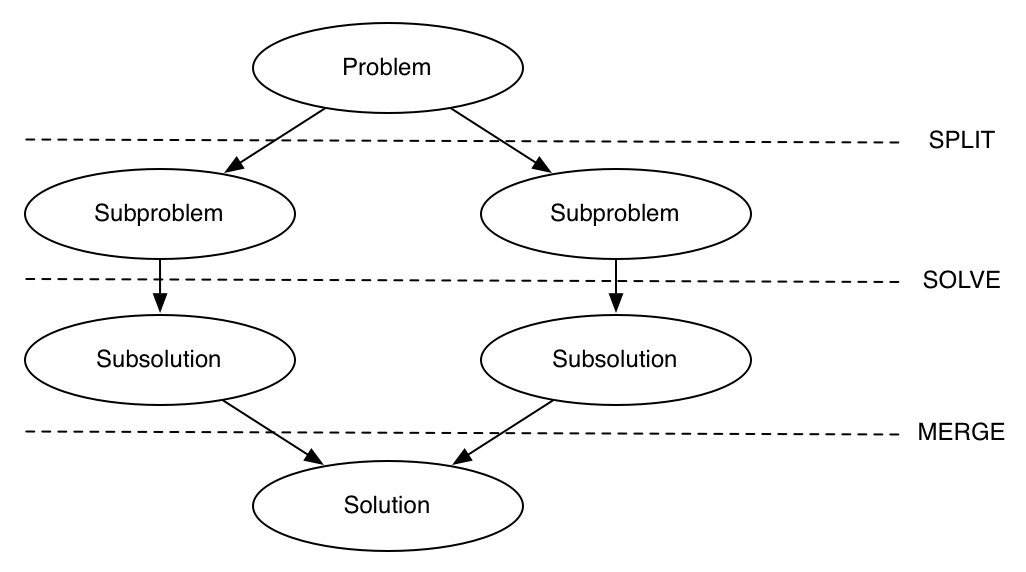
\includegraphics[width=\textwidth]{figsrc/DnC.png}
%     \caption{A diagram showing how divide and conquer works.\label{fig:DnC}}
% \end{figure}

\subsection{Main Contribution of This Dissertation}
\label{subsec:advantages}

\subsubsection{Reducing the Difficulty of Problems}

\subsubsection{Independence of Subproblems}

\subsubsection{Parallelism}


% Nowadays, a processor usually has multiple cores, and lots of computational tasks are implemented to be executed with parallel programs. In D\&C algorithm, the functions solving split subproblems are identically designed. With high independence and similar operations between subproblems, it is a good strategy to process them simultaneously. In other word, the original problem is suitable to be solved with \emph{SIMD (Single-Instruction-Multiple-Data)} parallel programs.

\chapter{Preliminaries}
\label{c:preliminaries}
In this section, common techniques of object detection are mentioned. Preprocessing (thresholding, color model transformation,blob detection) and recognition (feature point detection, and matching) are included.

\section{Common Image Processing Techniques}

    \subsection{Color Models}
        In this thesis, two color model were utilized to do the lettering defect detection and LED color \& function inspection.
        There is many different ways to describe colors in image processing.
        \subsubsection{RGB Color Model}
            The color model that most people known was 8 bits RBG color model.
            Which use 8 bits for each channel, could describe 256 X 256 X 256 colors.
            The idea of RGB color space is to separate colors to three primary color that human eyes could sense from light reflected from an object.
            By summing up three different color channel, we could simulate different colors in nature.
            Common used in color LED control and describing the color of a pixel.
            This color model is also the model used to describe raw image captured from camera we used.
        \subsubsection{Gray-scale}
            The color model we used to do lettering defect detection was 8 bit gray-scale color model, this color model could help us in production line to simply parameter setups.
            Also, gray-scale color model performs better then RGB to HSV color model when doing the lettering defect detecting.
            The conversion method from RGB color model to gray-scale color model built in OpenCV is described as below.
            % https://docs.opencv.org/3.1.0/de/d25/imgproc_color_conversions.html
            \begin{center}
            $ Y = 0.299 \times R + 0.587 \times G + 0.114 \times B $
            \end{center}

            Here is an example conversion result.
            \begin{figure}
                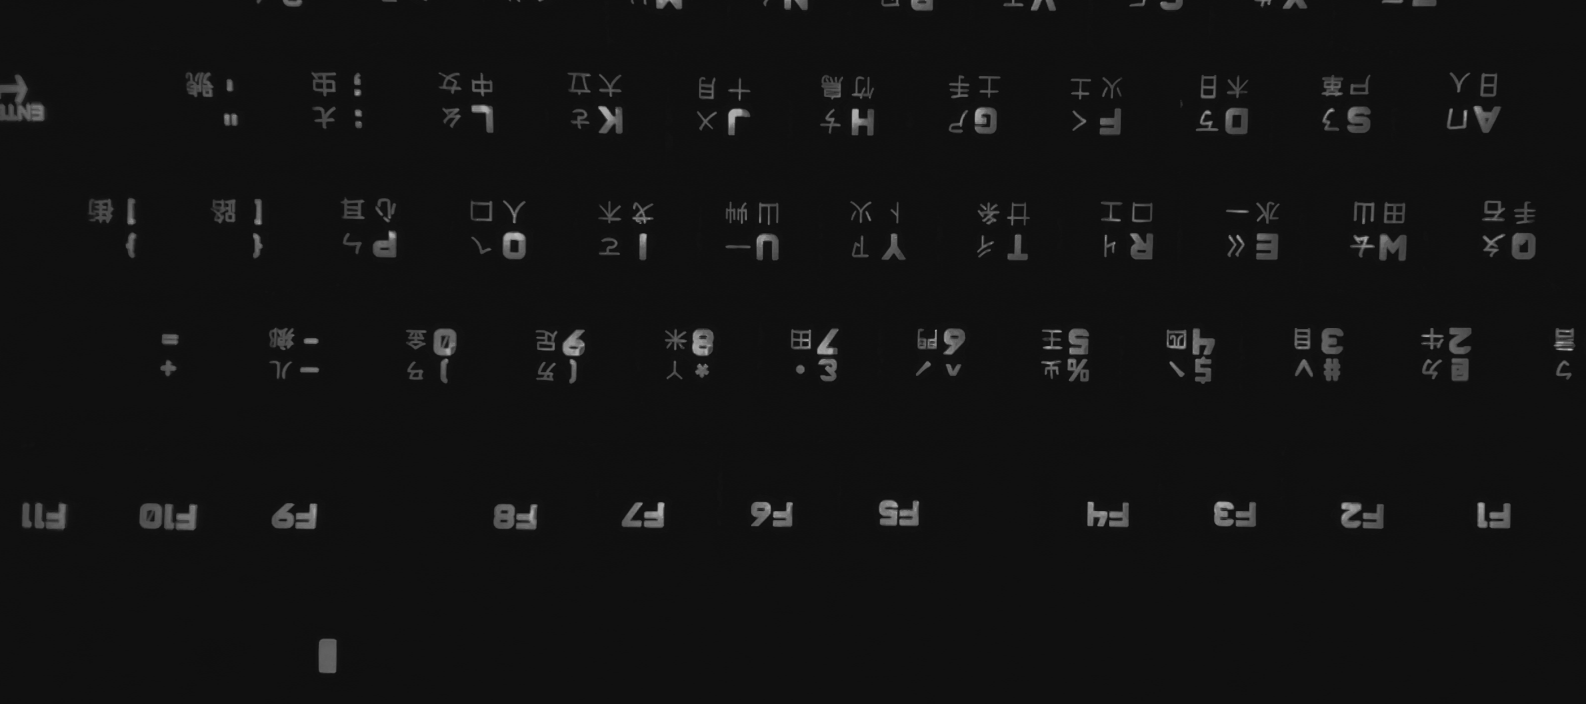
\includegraphics[width=\linewidth]{grayInput.png}
                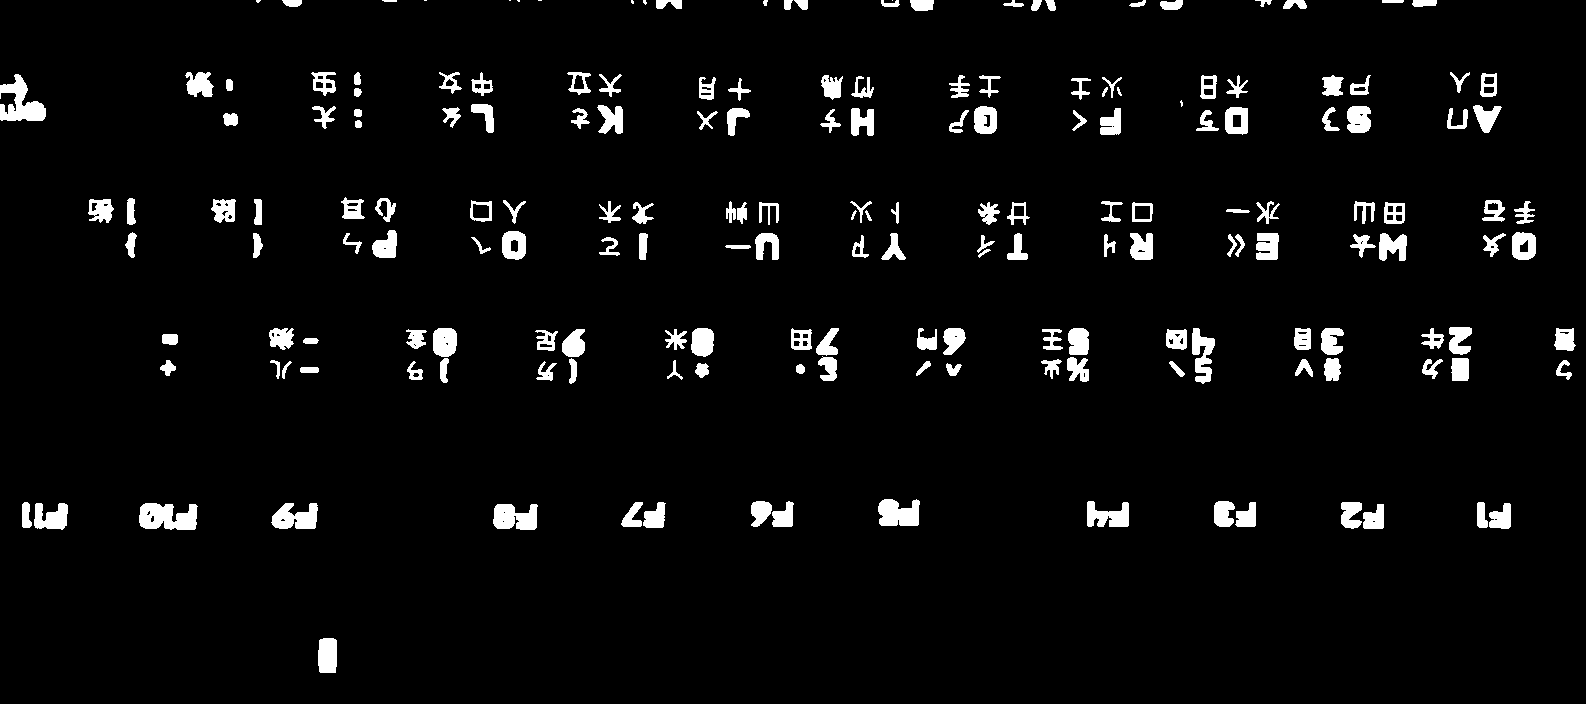
\includegraphics[width=\linewidth]{grayBinaryOutput.png}
                \caption{Grayscale thresholding example.}
                \label{fig:thresholding_Example}
            \end{figure}


        \subsubsection{HSV Color Model}
            The other color model we used was HSV color model, an alternative of RGB color model, this color model describe colors in different way of RGB color model.
            HSV color model use Hue, Saturation and Value to describe different colors.
            This color space could describe different color in a more intuitive way.
            Hue is the parameter represent for the color tone of the pixel. % find formal definition
            Saturation stands for how dense the color is. The more pure pixel color is, the higher value saturation will have.
            Value is used to describe how bright the pixel is. The brighter, the higher.
            The conversion method from RGB color model to HSV color model built in OpenCV is described as below.

            $$
                V = \max(R,G,B)
            $$\\
            $$
                S = 
                \begin{cases}   
                    {{{(V-min(R,G,B))}/{V}}, \enspace\textrm{if}\enspace V \neq 0}\\
                    {0, otherwise}
                \end{cases}
            $$\\
            $$
                H =
                \begin{cases} 
                    {{60(G - B)}/{(V-\min(R,G,B))}, \enspace\textrm{if}\enspace V=R}\\
                    {{120+60(B - R)}/{(V-\min(R,G,B))}, \enspace\textrm{if}\enspace V=G}\\
                    {{240+60(R - G)}/{(V-\min(R,G,B))}, \enspace\textrm{if}\enspace V=B}
                \end{cases}
            $$\\
            $$
                \textrm{If} \enspace H \enspace < \enspace 0 \textrm{, then } H = H + 360. \textrm{ On output } 0 \leq V \leq 1, 0 \leq S \leq 1, 0 \leq H \leq 360
            $$\\
            % \textrm{add HSV filtered example here} 
            \begin{figure}
                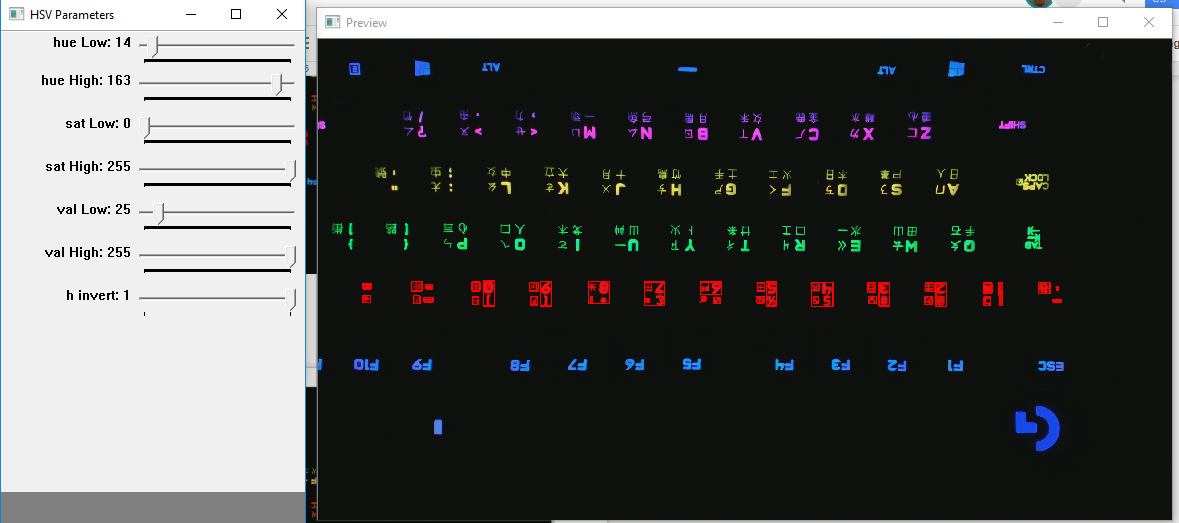
\includegraphics[width=\linewidth]{hsvRed.png}
                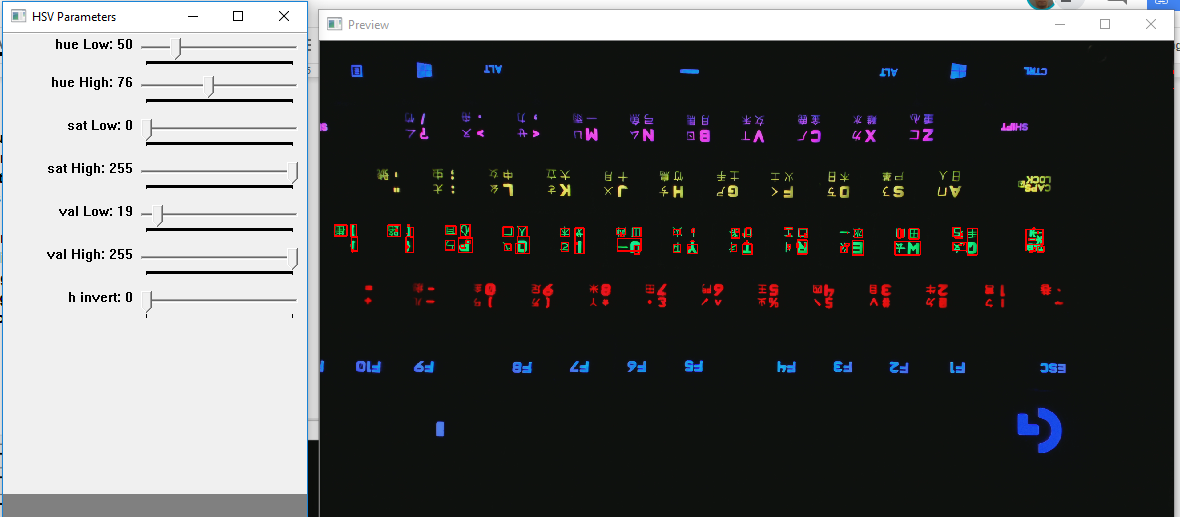
\includegraphics[width=\linewidth]{hsvGreen.png}
                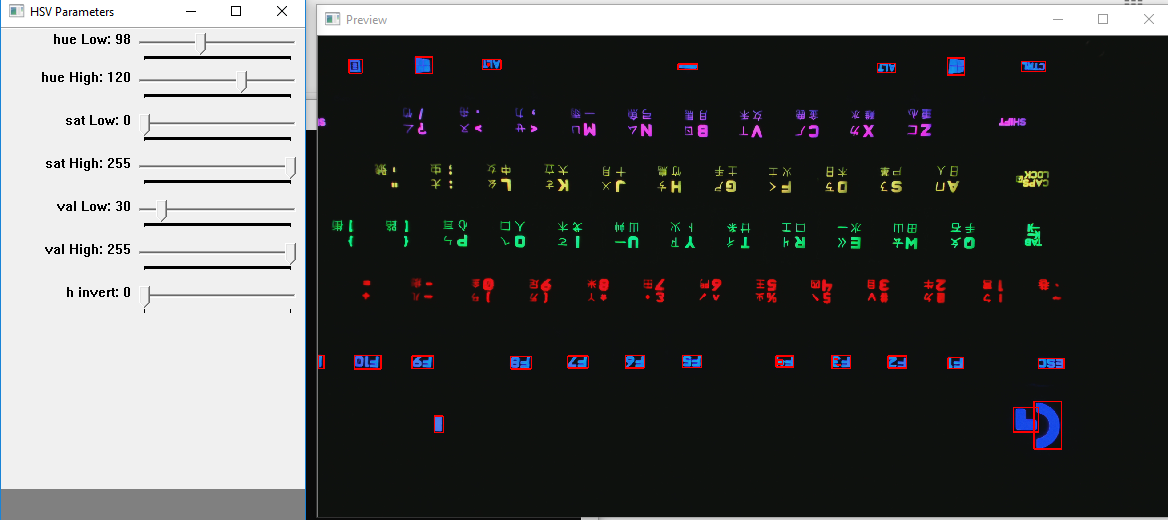
\includegraphics[width=\linewidth]{hsvBlue.png}
                \caption{HSV filtered examples. (RGB color detection)}
                \label{fig:HSV_Example}
            \end{figure}
`'
    \subsection{Thresholding \& Binarization}
        Thresholding with different color model can help us select interested pixels in an efficient way.
        In this thesis, we used this idea to identify where the keyboard buttons are located by doing thresholding to the gray scale image.
        By set a threshold value between 0 \& 255, we can get a binarized image.
        After apply blob or contour detection methods to that  binarized image.
        When thresholding with HSV upper bounds \& lower bounds, we can identify pixels with certain color or brightness.
        By HSV thresholding, we can identify keys with different color lightening.
        Witch is efficient for us to check if the LED back-light is malfunction.
        % add object detection, color detection, shape detection methods.
        $$ \textrm{add example here} $$

    \subsection{Blob Detection}
        % https://www.learnopencv.com/blob-detection-using-opencv-python-c/
        A blob is a group of connected pixels in an image that share some common property (e.g. gray-scale value, HSV value, RGB value, shapes, area, etc).
        The goal of blob detection method is to identify and mark these pixels in the given image.
        In this thesis, after we applied thresholding technique and defect detecting methods to the keyboard image captured from camera and get the corresponding binary image.
        We apply blob detection to that binary image then get the key position, LED color and defect information from it by apply blob detecting with different binary filters.
        $$ \textrm{add example here, grayscale thresholding, HSV filtering.....} $$

    \subsection{Feature Point Detection}
        Feature point detection technique is widely used in object detection or tracking applications.
        Popular methods like SIFT feature points having the current state of the art accuracy, but its slow on execution.
        SURF is an improve based on SIFT feature point. SURF is much faster then SIFT without sacrificing much robustness. But still takes some time when dealing with large sized image. 
        However, by restricting the area of interested with correct parameter setting, SURF feature point could be utilized in our project.
        Other feature point detecting methods like FAST, ORB and FREAK will also be discussed in Chapter 4.

\section{Related Works} 
    % Keywords: Planner object detection, Defect detection, AOI system.
    % this part needs more works to do later.
    % each subsection needs more information.
    This section will introduce where the main concept of each component comes from.
    \subsection{PCB defect detection}
        % https://ieeexplore.ieee.org/stamp/stamp.jsp?tp=&arnumber=5530052
        % defect detecting method referenced from this work.
        Putera et al., \cite{putera2010printed} (2010) proposed a computer vision inspection system implemented with MATLAB.
        The idea of updated defect detection method for keyboard lettering is from this work.

    \subsection{Computer-Vision-Based Fabric Defect Detection}
        % https://ieeexplore.ieee.org/stamp/stamp.jsp?tp=&arnumber=4418522
        % where multiple camera idea from
        Kumar et al.,(2008)\cite{kumar2008computer} gives a design of CV based inspection platform for fabric defect detecting.
        We applied the idea connect multiple camera to one host machine in this thesis.

    \subsection{Image Alignment}
        % https://www.learnopencv.com/image-alignment-feature-based-using-opencv-c-python/
        % https://www.learnopencv.com/image-alignment-ecc-in-opencv-c-python/
        On the website owned by Satya Mallick, he showed two different way to do the image alignment.
        One is by enhanced correlation coefficient (ECC) \cite{ECC_Alignment}, the other is based on feature point matching \cite{featureBasedAlignment}.

\section{Previous Solution}
    % give more detailed introduction on previous solution.
    Previous solution applied SURF feature point on every ROI that represented a key, and we found that feature point based method have accuracy issue on small target searching at production line.
    Also, the lettering defect detecting method is not sensitive enough to deal with small defect.
    In this thesis, we'll focus on how to correct these problems.
\chapter{Methods}
\label{c:methods}

\section{Inspection Platform Structure}
Refer to Kumar's work \cite{kumar2008computer}, we designed a scalable platform could install multiple cameras. Use one PC as host machine to collect images from camera array.
After retrieved images from camera, the defect detection methods (Lettering Defect Detection \& LED Color inspection) described below will inspect wheather the keyboard has any defect on it. 
\begin{figure}
	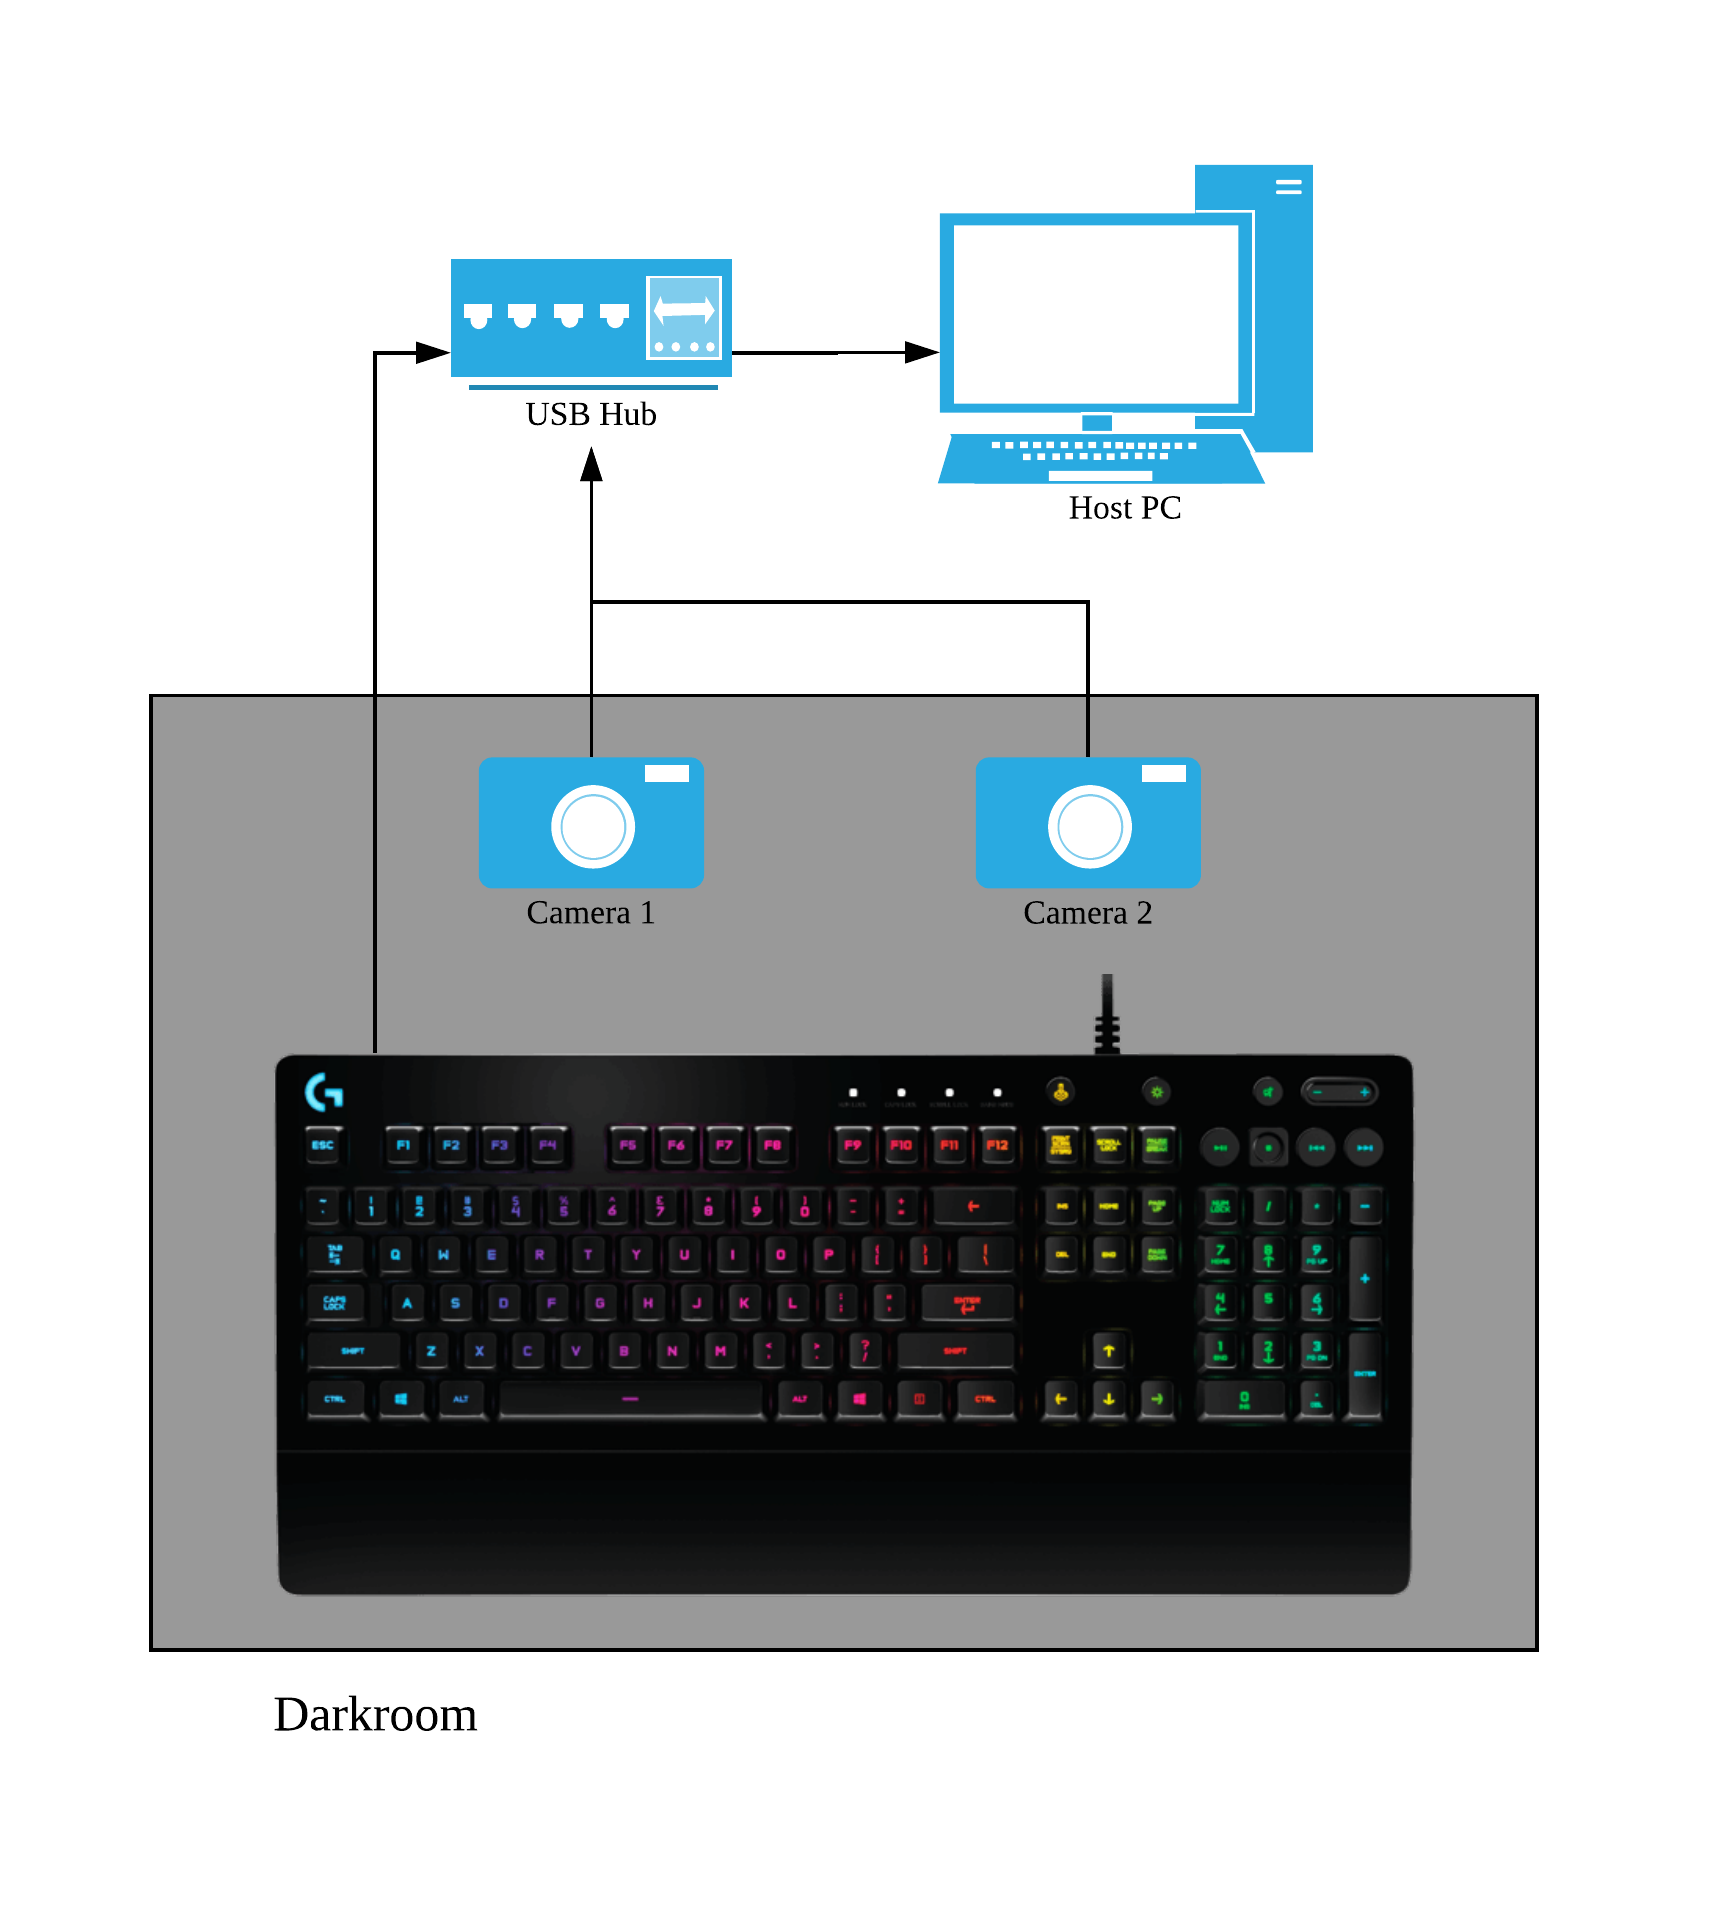
\includegraphics[width=\linewidth]{SystemStructure.png}
	\caption{The Diagram of SystemStructure}
	\label{fig:SystemStructure}
\end{figure}


\section{Lettering Defect Detection Intorduction}
\label{letteringDetection}
	In lettering defect detection, we want to check the layout of keyboard and quality of laser engraving on each key.
	We'll give a detailed explan of how the lettering defect detection is designed and how they work.

	\subsection{Learning Stage} 
		Lettering defect detection can be saperated into two main part.
		The first part is learning stage. This part reads the gold image from file and doing the feature point detection, and store the feature points \& their descriptor for examining stage use.

		\begin{figure}
			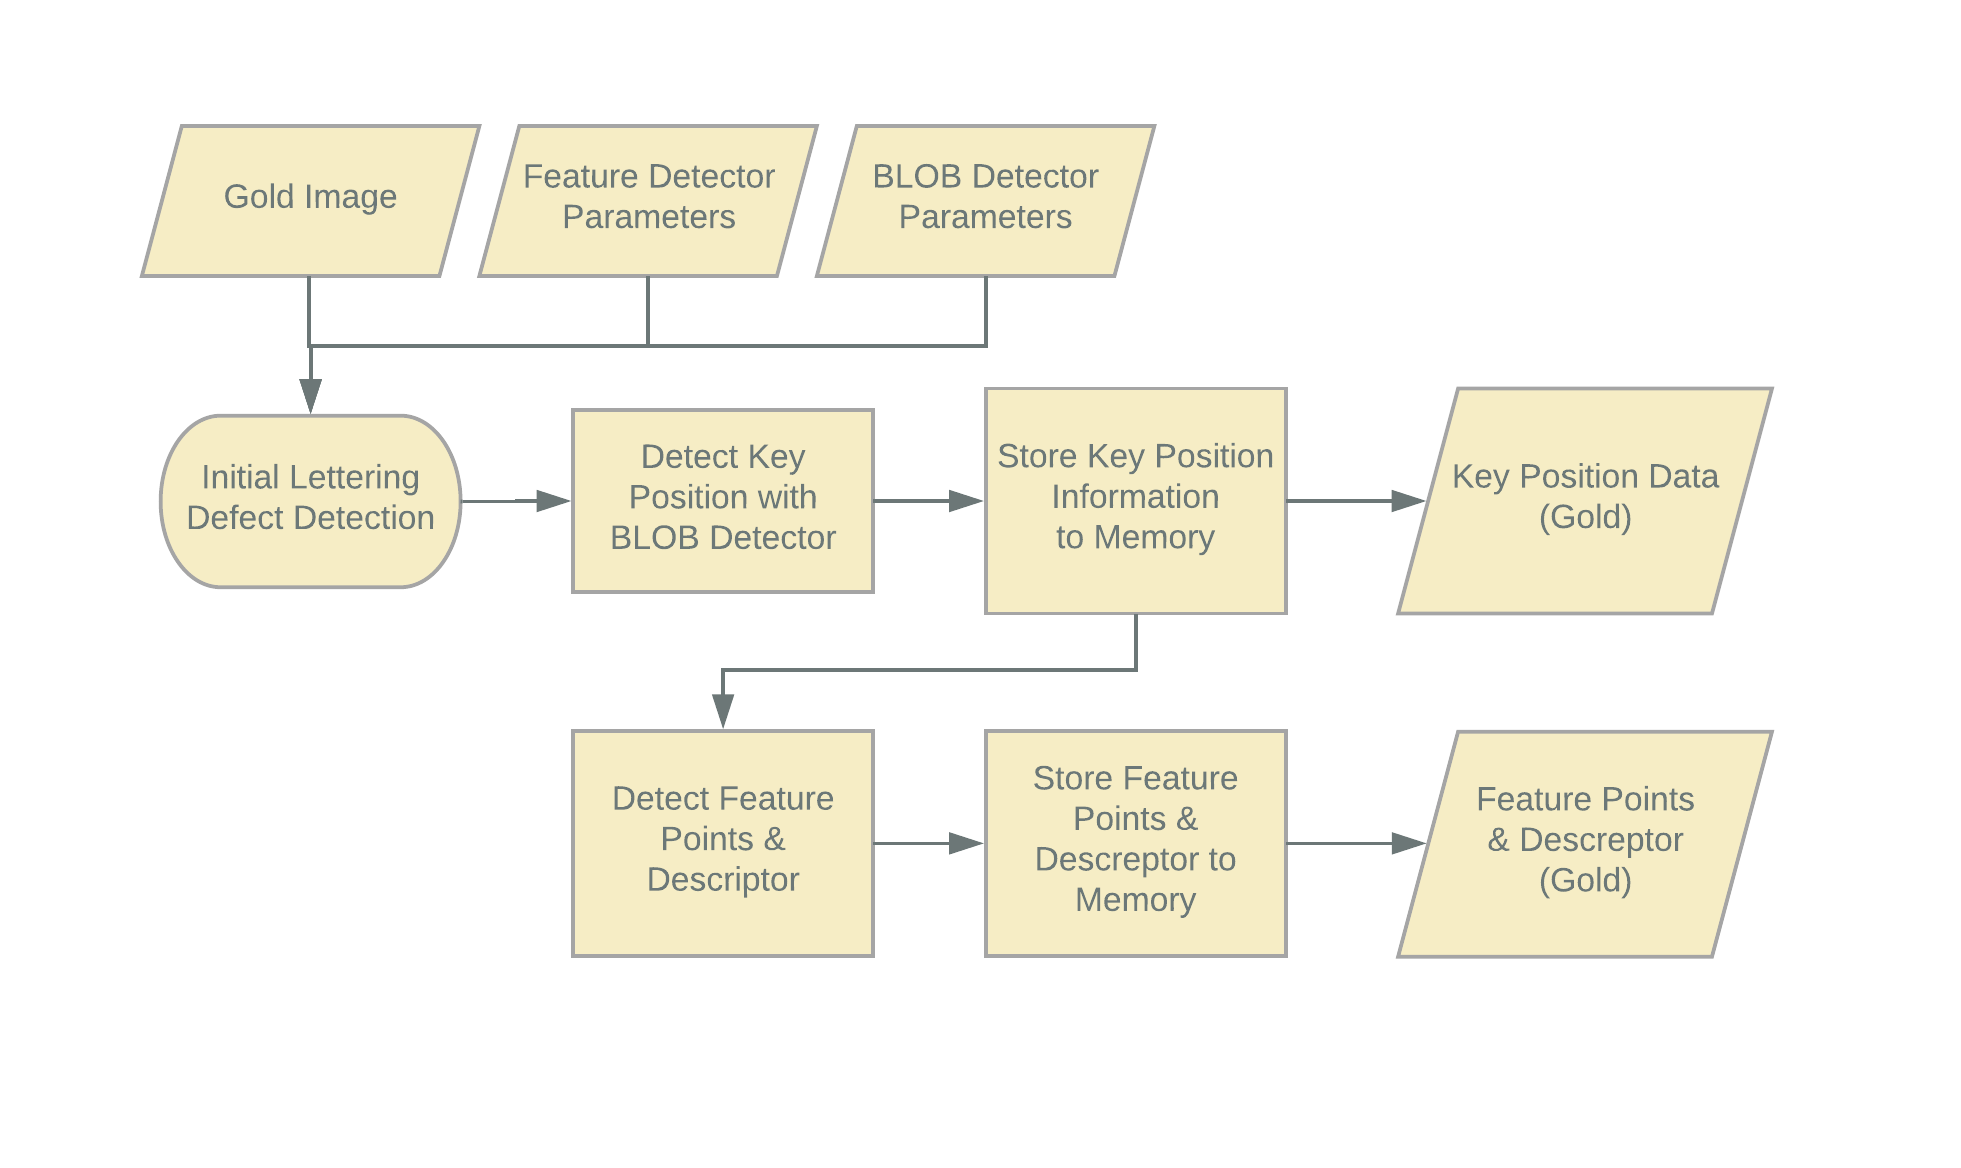
\includegraphics[width=\linewidth]{LetteringInit.png}
			\caption{The Diagram of Lettering Initialize Stage}
			\label{fig:LetteringInit}
		\end{figure}

	\subsection{Inspection Stage}
		In lattering examing stage, we did same steps on the keyboard sample image we want to imspect, doing the feature point detection and store the feature points \& their descriptor.
		After having the feature point and descriptor from both gold \& keyboard sample image, we do the feature point matching to find the homography matrix then we can align sample image with gold image with geomatric transformantion. 
		With both image aligned, we apply the defect detection method to aligned images, and get the marked defect information.
		And judge the sample keyboard is a defected on or a good one.
		\begin{figure}
			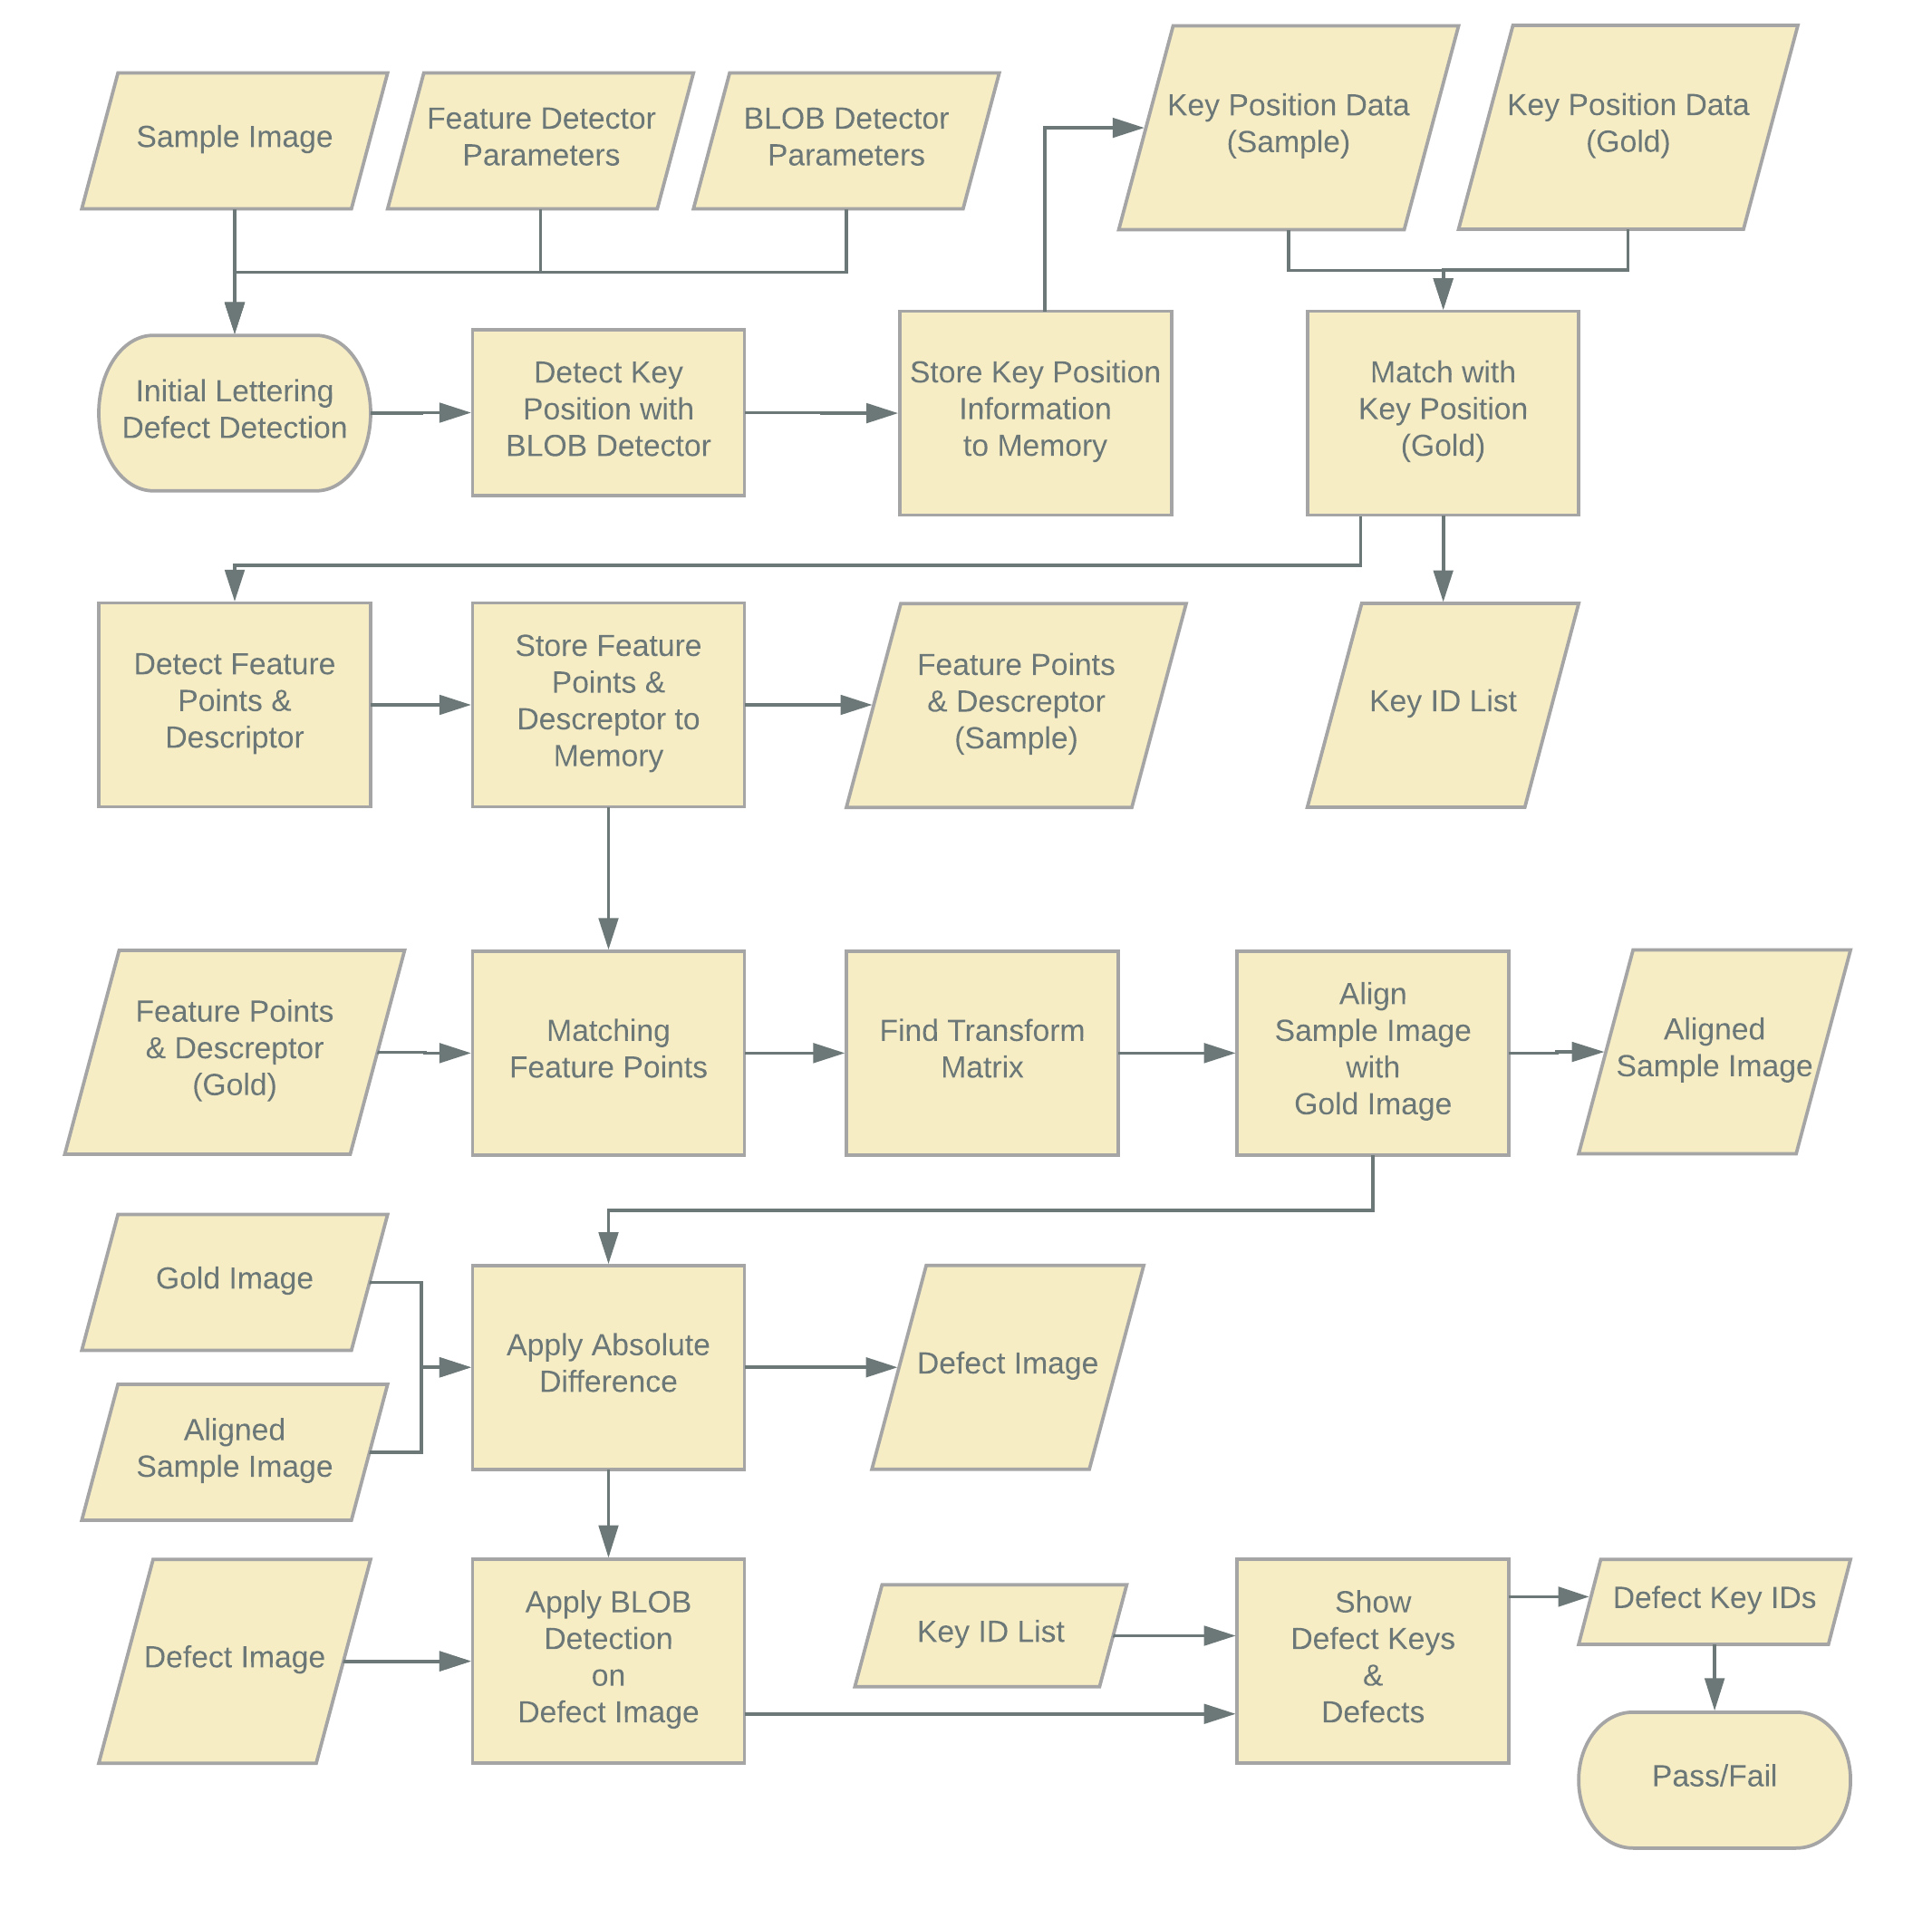
\includegraphics[width=\linewidth]{LetteringInspection.png}
			\caption{The Diagram of Lettering Inspection Stage}
			\label{fig:LetteringInspection}
		\end{figure}

	\subsection{Defect Detection Method}
		In lettering defect detection, after gray-scale gold \& smaple image aligned, we calculate absolute difference of two image, and get a new gray scale image, say $M_{Diff}$, that contained defects information.
		To detect the defect, we could apply simple blob detection with soutable parameters to identify wheather a bright spot is defect or noise.
		
		$$ \textrm{add a flow chart here} $$
		$$ \textrm{add example image of absdiff result after alignment} $$

\section{LED Mulfunction Detection Intorduction}
	In LED function inspection, we want to check if each LED embadded in the circuit of keyboard functions as expect.
	In this stage, we'll capture three pair of gold and sample image, $(gold_R, sample_R), (gold_G, sample_G), (gold_B, sample_B)$, used to inspect three different color chanel of LED light source.
	The detailed method will be described in following subsectinos.
	\subsection{Learning Stage}
		In this step, we want to build the pass standard with given gold image.
		By apply corresponding HSV filter, $filter_r, filter_g, filter_b$, to gold images, we can obtain three binary image, witch can use to identify if a testing object funcions as this binary image.
		\begin{figure}
			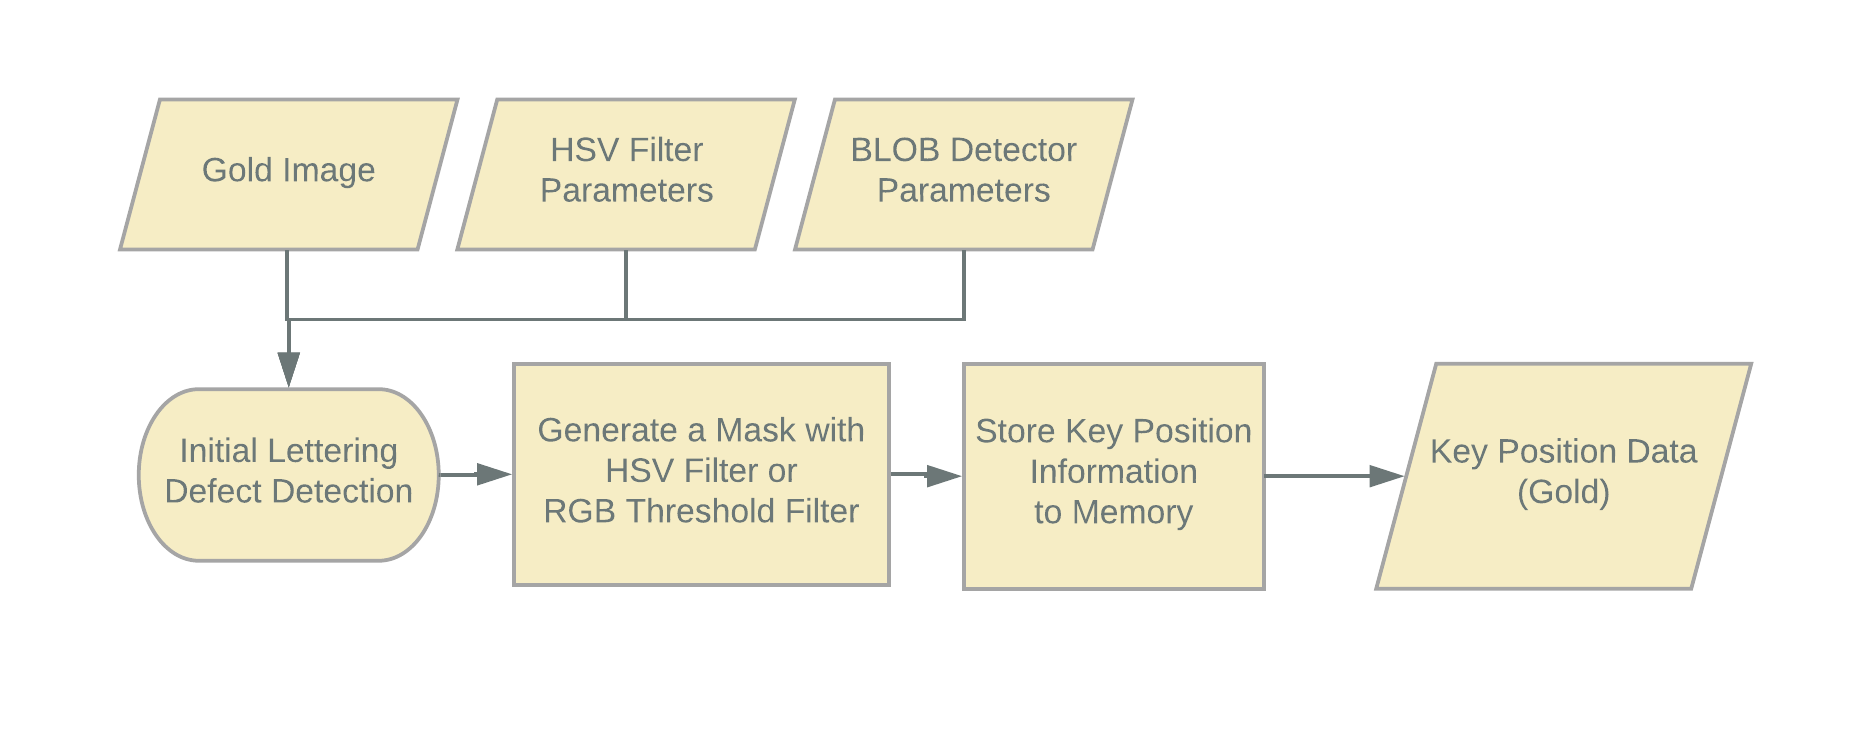
\includegraphics[width=\linewidth]{LEDInit.png}
			\caption{The Diagram of LED Initialize Stage}
			\label{fig:LEDInit}
		\end{figure}

	\subsection{Inspection Stage}
		In this step, we are going to check if a testing object functions as the passing standard.
		We applied same filter, say $filter_c$, on the image captured from camera. And get a binary image of testing object.
		We compare the blob size and shape between the binary image of gold and sample, to see if there is any mulfunctioning on the LED lights.
		\begin{figure}
			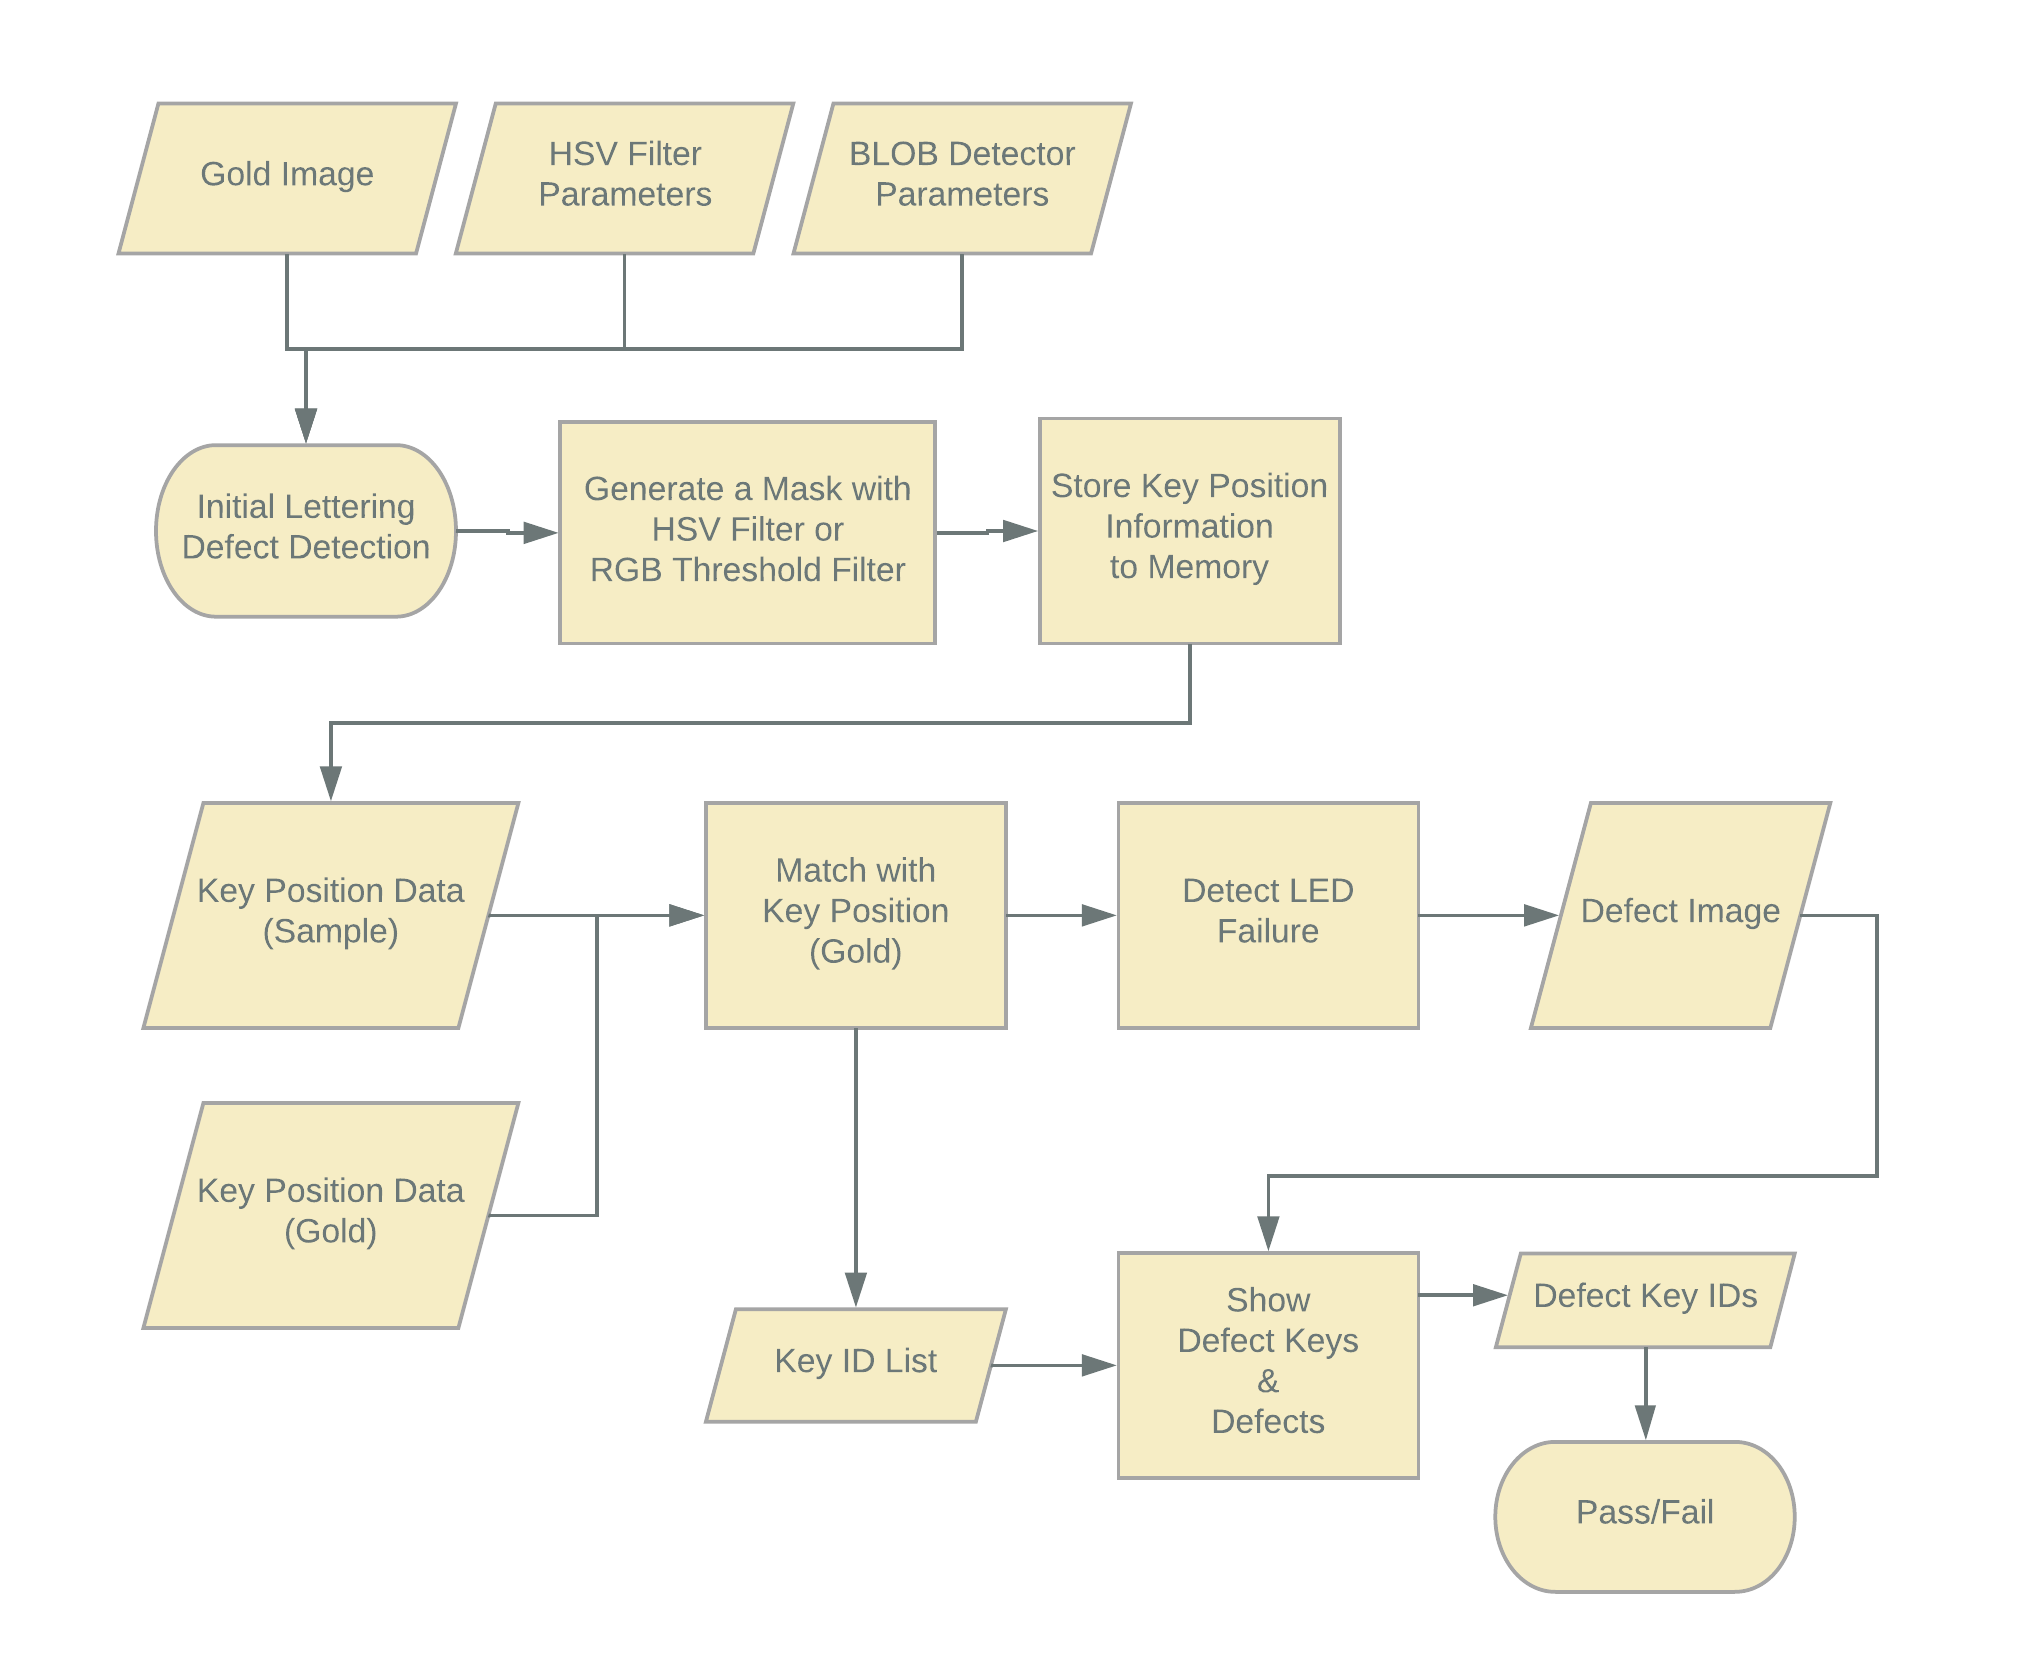
\includegraphics[width=\linewidth]{LEDInspection.png}
			\caption{The Diagram of LED Inspection Stage}
			\label{fig:LEDInspection}
		\end{figure}

\section{Other Functions Implemented}
	\subsection{Stamp Detection}
		Stamp detection is implemented after lattering defect detection is implemented.
		Since the steps doing object detection and feature based image alignment are very similar.
		We first applied feature point detect method on the stamp image and image that we want to inspect.
		After applied point matching methods, we could find the posible area for the stamp.
		Finally, we compare the similarity between the posible area, make sure that there is no misjudge on the inspection.
\chapter{Comparision Between Other Mehtods}
\label{c:comparision}
\chapter{Conclusions \& Future Works}
\label{c:conclusion-and-future-works}

\section{Conclusions}
	
\section{Future Works}
	\subsection{Ability To Inspect Non-illuminated Keyboards}
	\subsection{Multicamera controls optimizatin}
	\subsection{GPU is not utilized in this project}
	\subsection{Smarter Algorithm}
\appendix

\backmatter

\renewcommand{\bibname}{References}
\addcontentsline{toc}{chapter}{\bibname}
\bibliographystyle{ieeetr}

% Your bibliography goes here
{\singlespacing
\bibliography{thesis}
}

\end{document}
